\chapter{Functional and Non-Functional Requirements}\label{app:requirements}

The complete list of requirements, with a one-sentence summary and the prototype status of each, is kept with the source code:

\begin{center}
\url{https://github.com/rawdatarekkkk/jadwai/blob/main/docs/REQUIREMENTS.md}
\end{center}

It is derived from the project's Software Requirements Specification (SRS) v0.4 of 18 November 2026, which defines the inputs, outputs, error behaviour and acceptance criteria of every requirement. SRS v0.2 was reviewed by the supervisor; v0.3 and v0.4 carry the project owner's approval only. The status is the owner's record of the prototype on 23 November 2026, not a supervisor acceptance or a research result: \emph{implemented} means working in the prototype with automated tests, \emph{partial} that a working subset exists.

\section{Functional requirements}

Table~\ref{tab:fr-areas} groups the 78 functional requirements by area. Of these, 55 are implemented, 17 partly implemented and 6 not started.

\begin{longtable}{@{}p{0.26\textwidth}p{0.17\textwidth}p{0.155\textwidth}p{0.33\textwidth}@{}}
\caption{Functional requirements by area.}\label{tab:fr-areas}\\
\toprule
Area & Requirements & Status & Main gaps \\
\midrule
\endfirsthead
\toprule
Area & Requirements & Status & Main gaps \\
\midrule
\endhead
Term data and records & FR-001--FR-008 & Partial & One term only; no aliases or dated availability exceptions \\
Constraint vocabulary and lifecycle & FR-009--FR-013 & Partial & No supersession history or weight editing \\
AI extraction and review & FR-014--FR-023, FR-073, FR-074 & Partial & Extraction quality not yet measured; no audit export with cost \\
Scheduling & FR-024--FR-030, FR-065--FR-070 & Implemented & --- \\
Validation & FR-031--FR-033 & Implemented & --- \\
Scenarios and editing & FR-034--FR-039 & Partial & No explicit-variation scenarios (FR-037) \\
Publication and views & FR-040--FR-043, FR-078 & Implemented & --- \\
Export & FR-044, FR-045 & Implemented & --- \\
Traceability, accounts, audit & FR-046--FR-048 & Partial & Partial requirement-to-publication trace \\
Evaluation support & FR-049, FR-050 & Partial & No human annotations; no participant study \\
Examinations & FR-051, FR-071, FR-072 & Implemented & --- \\
Ask JAI & FR-075--FR-077 & Implemented & --- \\
Infeasibility explanation & FR-058 & Implemented & --- \\
Extensions & FR-052--FR-057 & Mostly not started & Arabic extraction (FR-054) works but is unmeasured \\
Exception handling & FR-059--FR-064 & Partial & Cancelled results are not retained \\
\bottomrule
\end{longtable}

\section{Non-functional requirements}

The SRS defines 23 non-functional requirements and invents no numeric targets; values that depend on later decisions remain open. Table~\ref{tab:nfr} summarises them.

\begin{longtable}{@{}p{0.19\textwidth}p{0.17\textwidth}p{0.56\textwidth}@{}}
\caption{Non-functional requirements and prototype status.}\label{tab:nfr}\\
\toprule
Category & Requirements & Status \\
\midrule
\endfirsthead
\toprule
Category & Requirements & Status \\
\midrule
\endhead
Correctness & NFR-001--003 & Met in tests: separate validator; publication refused on any violation; a time limit is never reported as infeasibility \\
Security & NFR-004, 005 & Server-side permissions; no secrets in the repository. Passwords use scrypt instead of the specified Argon2id (recorded deviation) \\
Privacy & NFR-006, 007 & With the local model no text leaves the server; applicable data-protection rules still to be confirmed \\
Accessibility & NFR-008 & Labelled, keyboard-operable controls; no formal audit \\
Reliability & NFR-009, 010 & Timeouts, retries, malformed output and cancellation tested; recovery objectives open \\
Performance and scale & NFR-011--013 & Runtime, outcome and tested scale recorded with every result; no numeric targets \\
Usability & NFR-014, 015 & Checked manually; not measured (no participant study) \\
Reproducibility & NFR-016 & Versions, seeds and dates recorded for runs and fine-tuning \\
Maintainability & NFR-017 & Separate modules; model provider chosen by configuration \\
Compatibility, retention, backup & NFR-018--020 & Open; local backups before destructive changes \\
Localisation & NFR-021 & English and Arabic interface with right-to-left layout; mixed Arabic/English text kept in reading order \\
Observability, licensing & NFR-022, 023 & Partial; licence list not yet checked \\
\bottomrule
\end{longtable}

\chapter{Screenshots of the Prototype}\label{app:screenshots}

The following screenshots were taken from the running prototype on 23 November 2026 in the demonstration workspace (a browser window of 1440$\times$900 pixels). All names of people are demonstration placeholders. Further screenshots are in the repository folder \texttt{docs/screenshots}.

\begin{figure}[p]
\centering
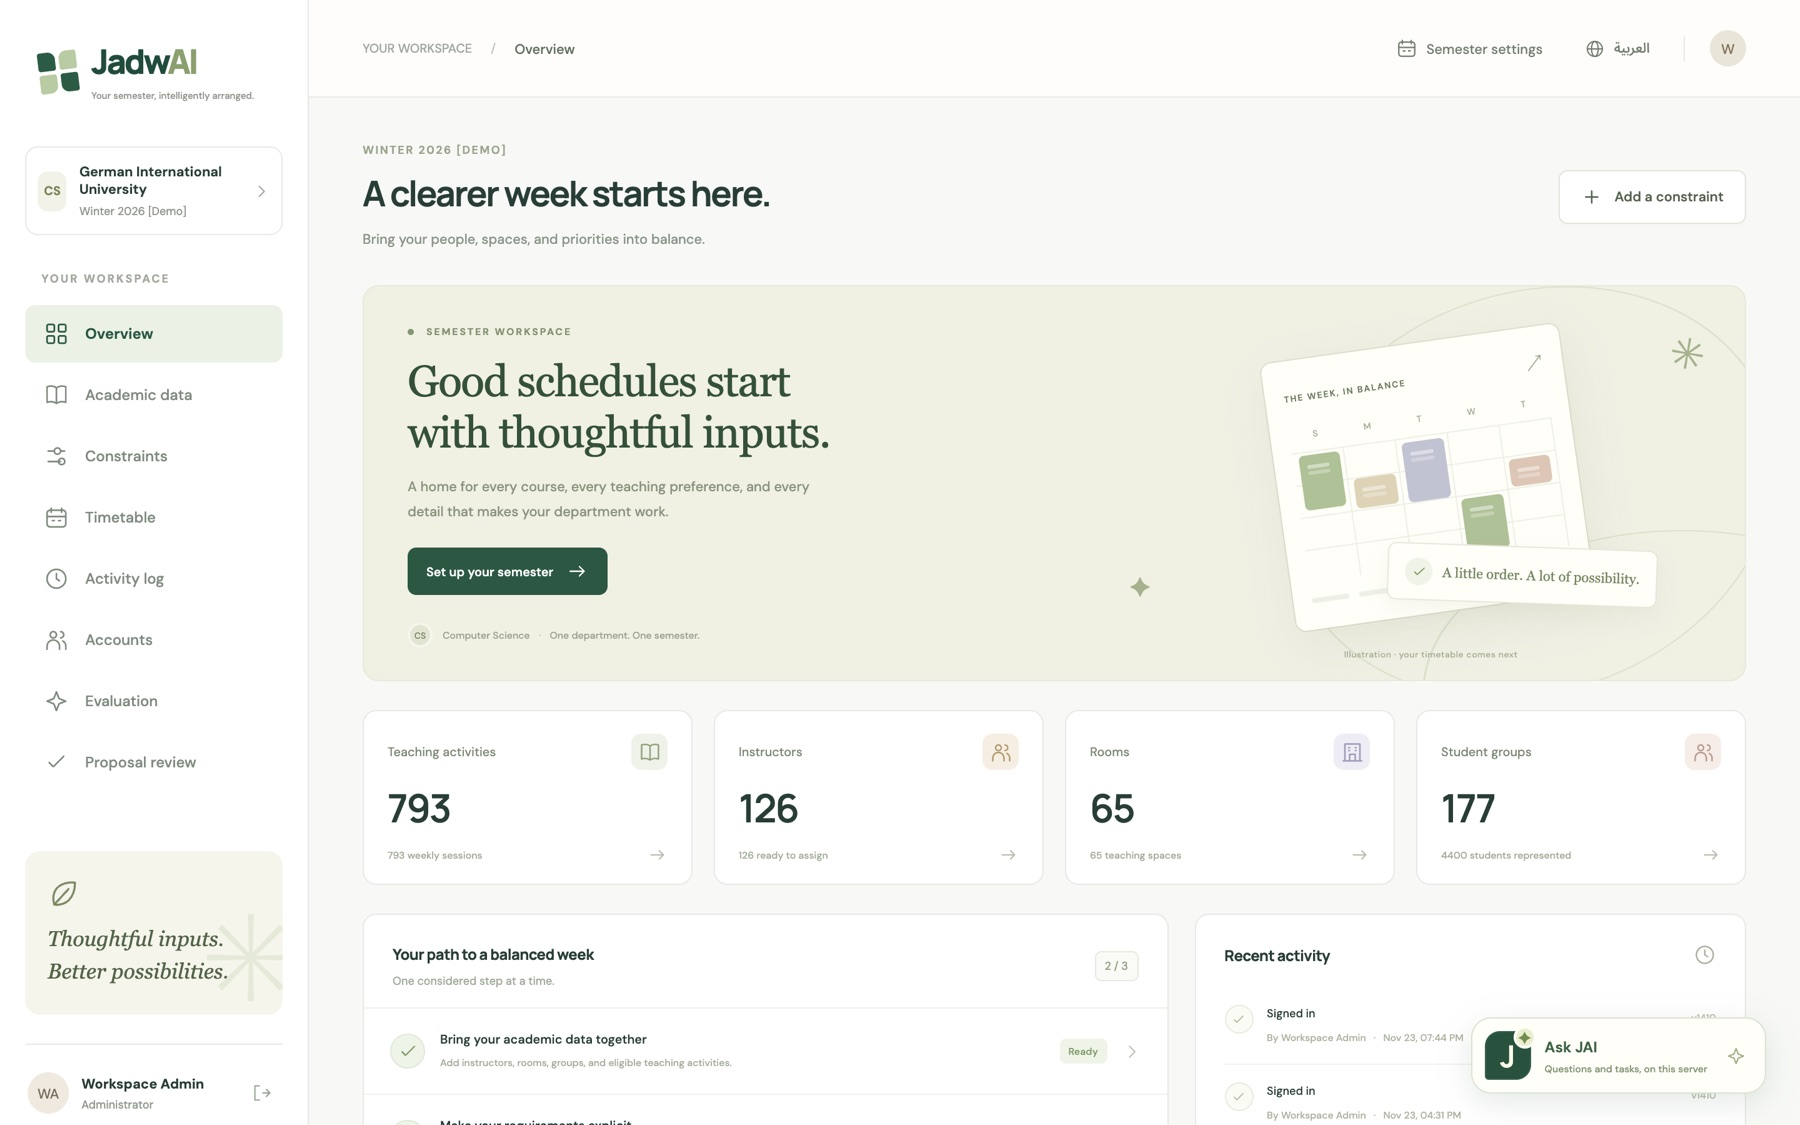
\includegraphics[width=\textwidth]{02-overview.jpg}
\caption{Overview page of the administrator workspace: counts of activities, instructors, rooms and student groups, the setup path and recent activity.}
\label{fig:shot-overview}
\end{figure}

\begin{figure}[p]
\centering
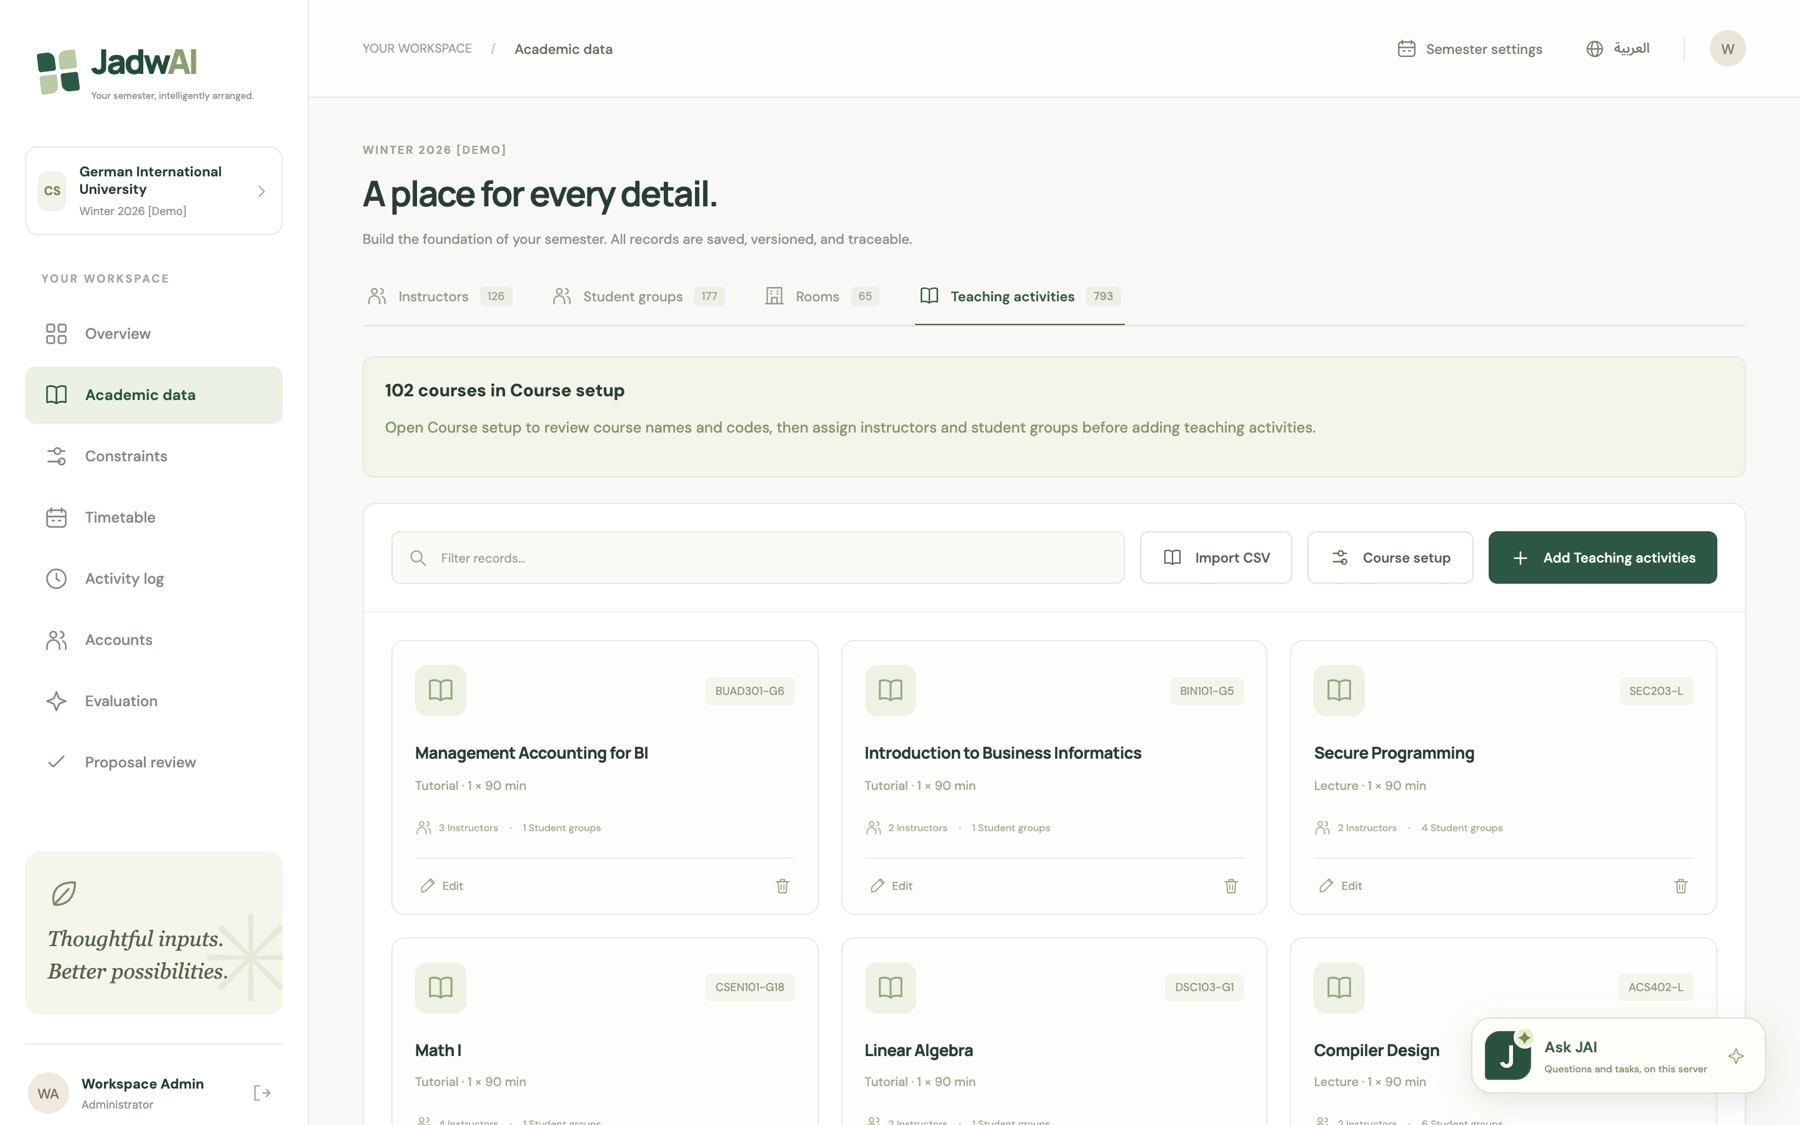
\includegraphics[width=\textwidth]{03-academic-data.jpg}
\caption{Academic data: teaching activities of each course, with separate tabs for instructors, student groups and rooms, and CSV import.}
\label{fig:shot-academic-data}
\end{figure}

\begin{figure}[p]
\centering
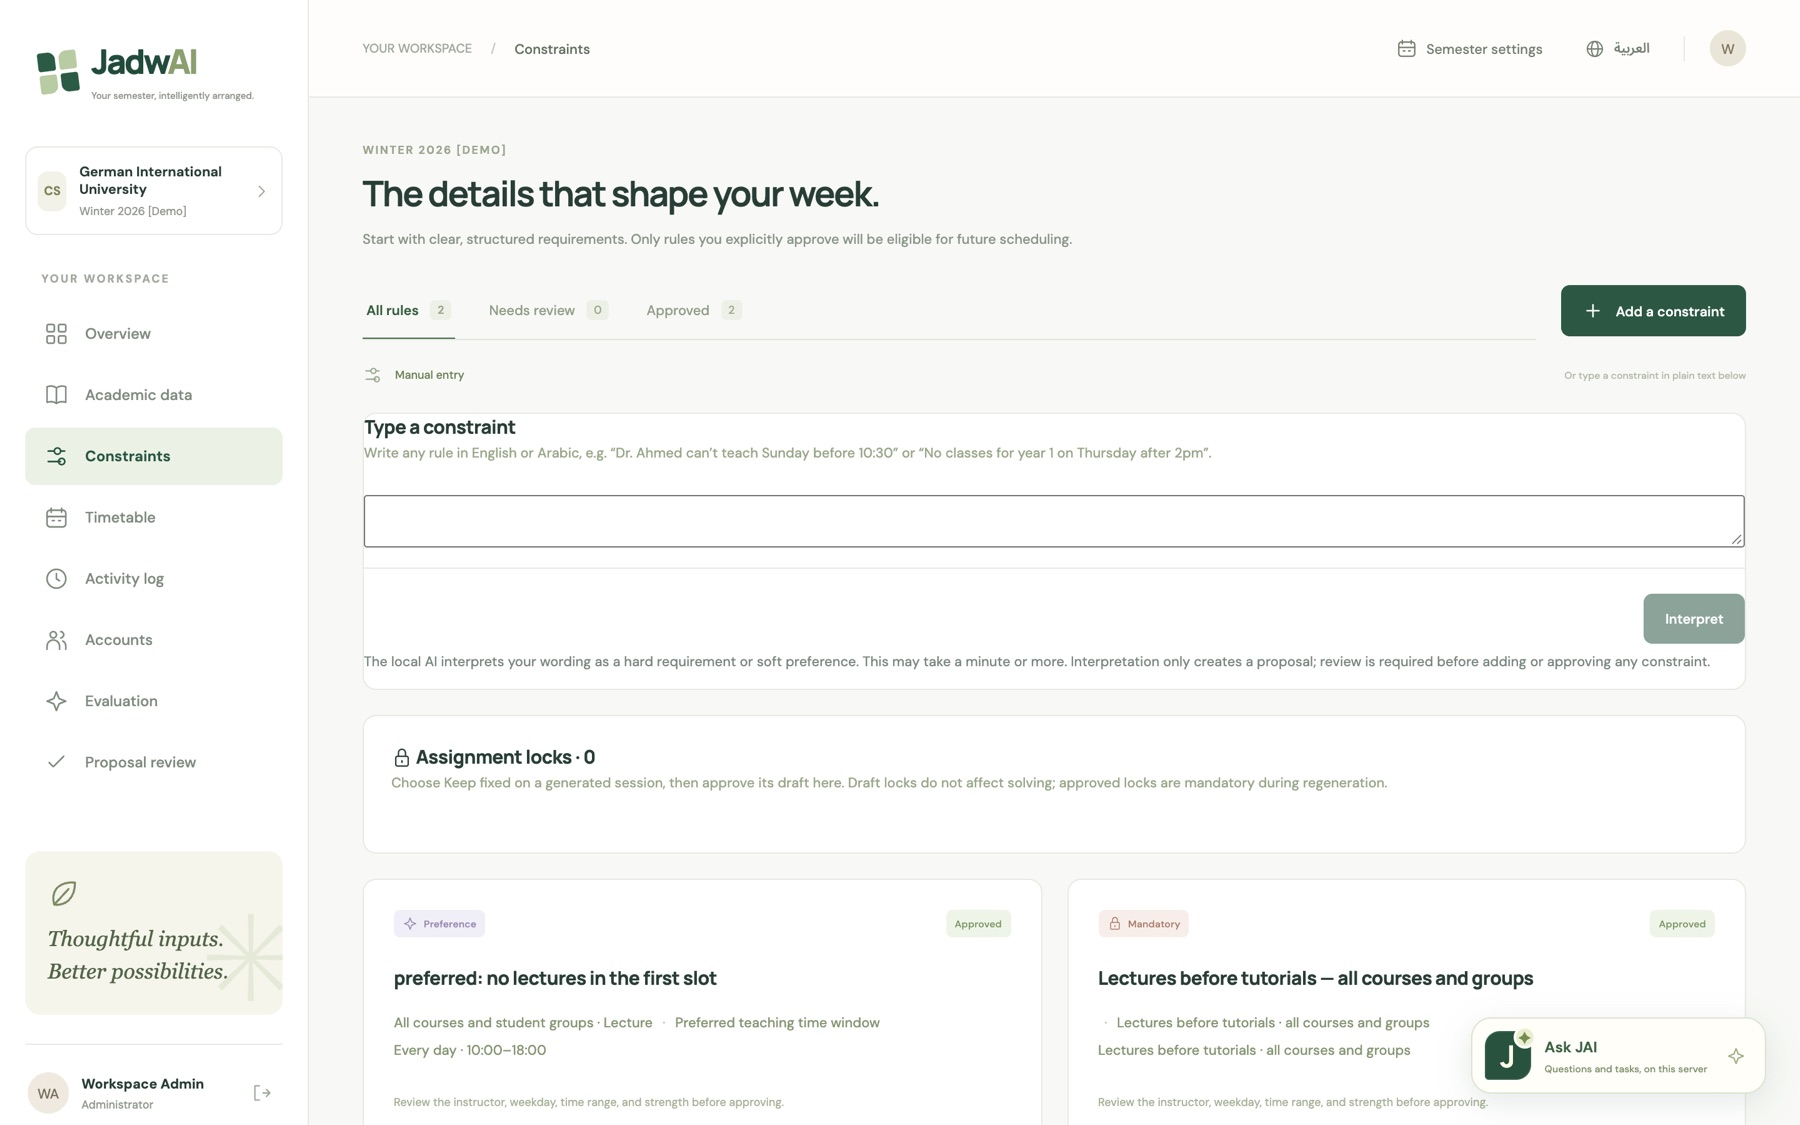
\includegraphics[width=\textwidth]{04-constraints.jpg}
\caption{Constraints: a requirement can be typed in English or Arabic and is interpreted as a proposal; approved rules are listed below with their strength (preference or mandatory).}
\label{fig:shot-constraints}
\end{figure}

\begin{figure}[p]
\centering
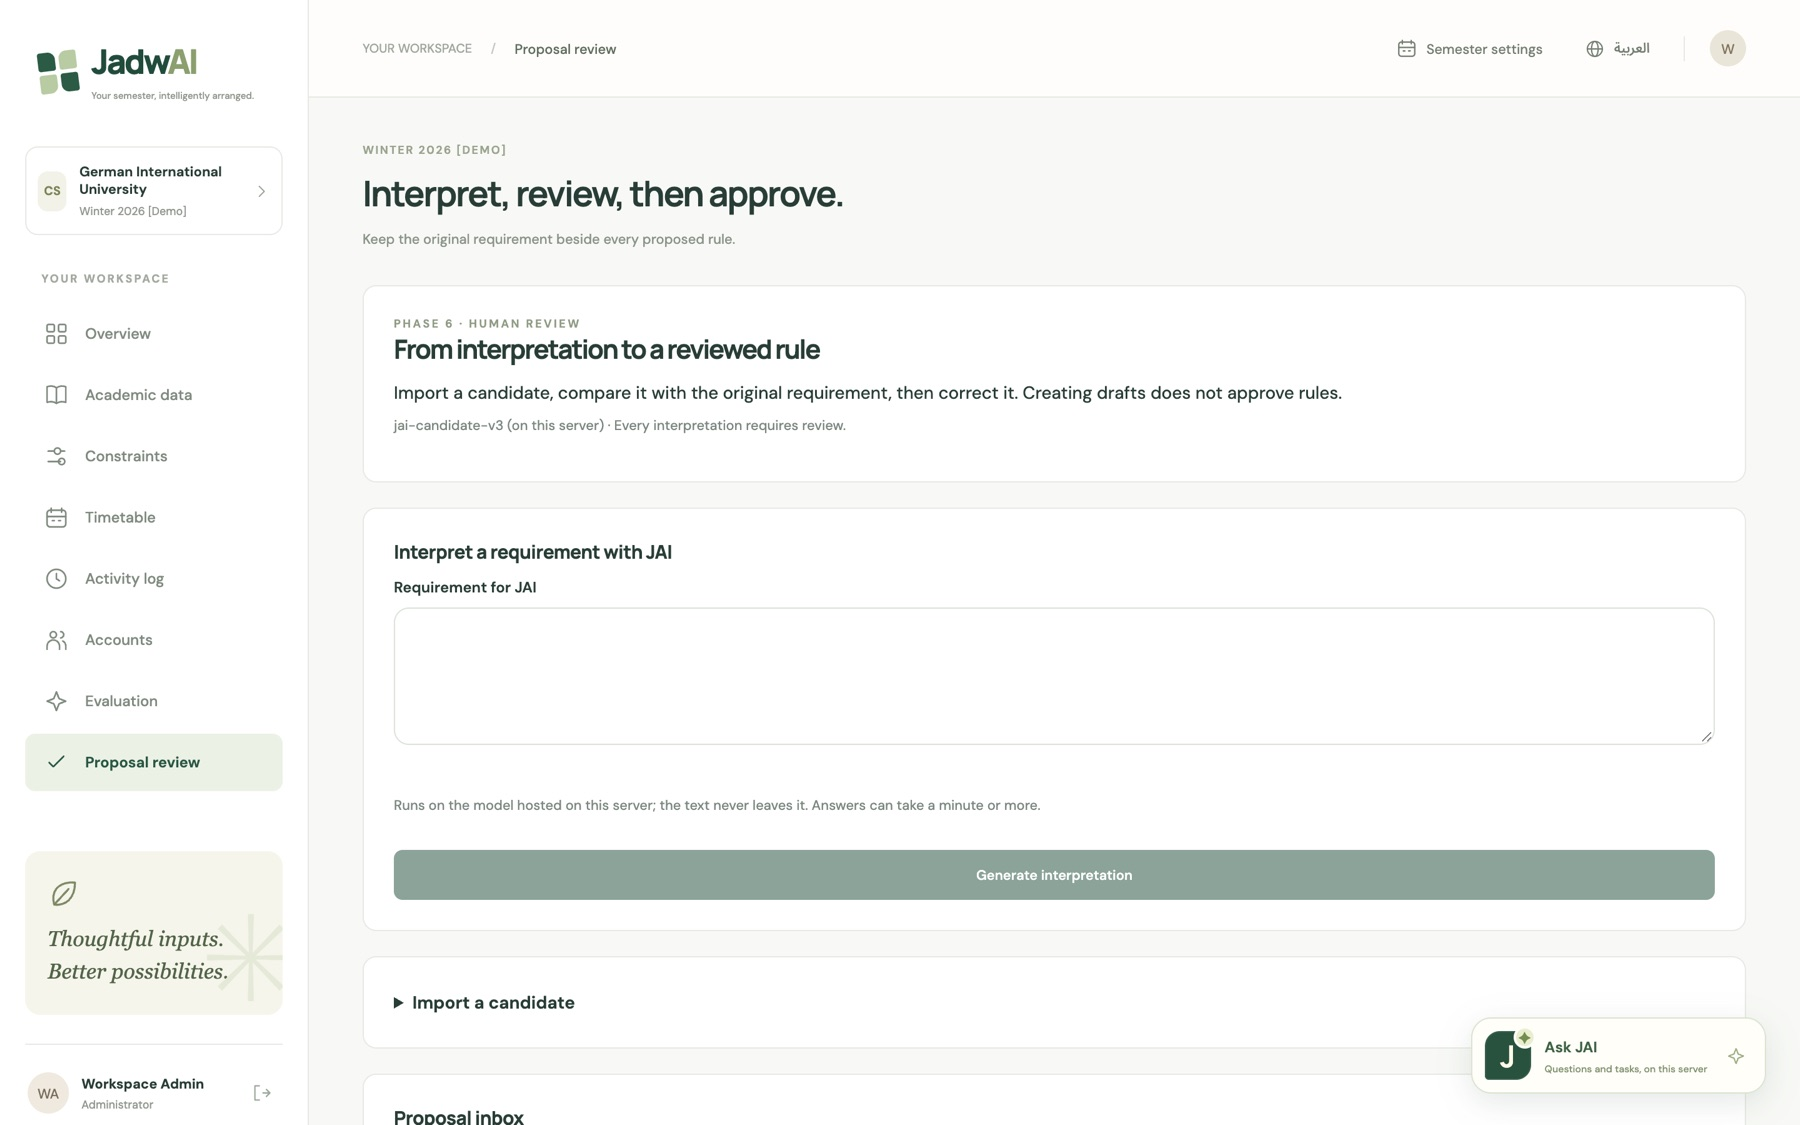
\includegraphics[width=\textwidth]{09-proposal-review.jpg}
\caption{Proposal review: a requirement is interpreted by the locally hosted model and shown beside the original text for correction before any rule is created.}
\label{fig:shot-proposal-review}
\end{figure}

\begin{figure}[p]
\centering
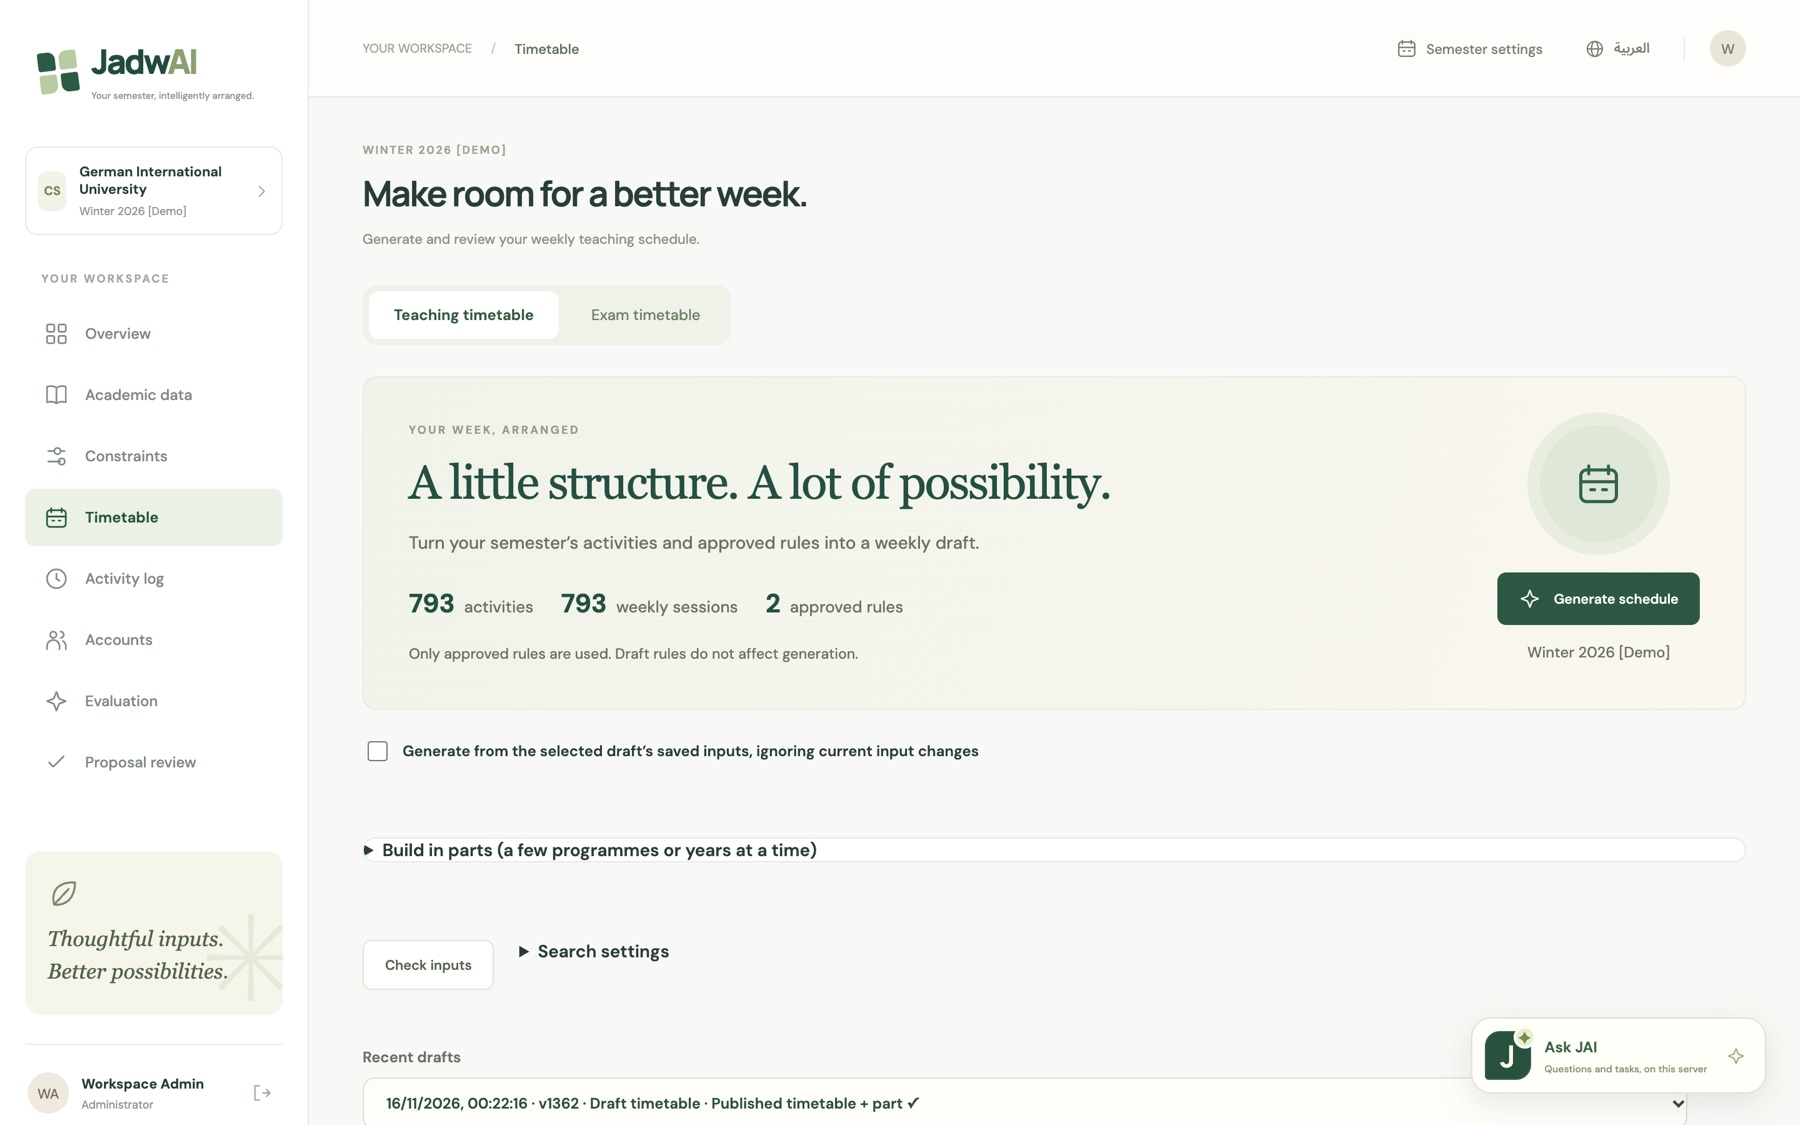
\includegraphics[width=\textwidth]{13-teaching-timetable-top.jpg}
\caption{Teaching timetable: generation from approved rules only, building in parts, input checks, search settings and the list of saved drafts.}
\label{fig:shot-teaching-timetable-top}
\end{figure}

\begin{figure}[p]
\centering
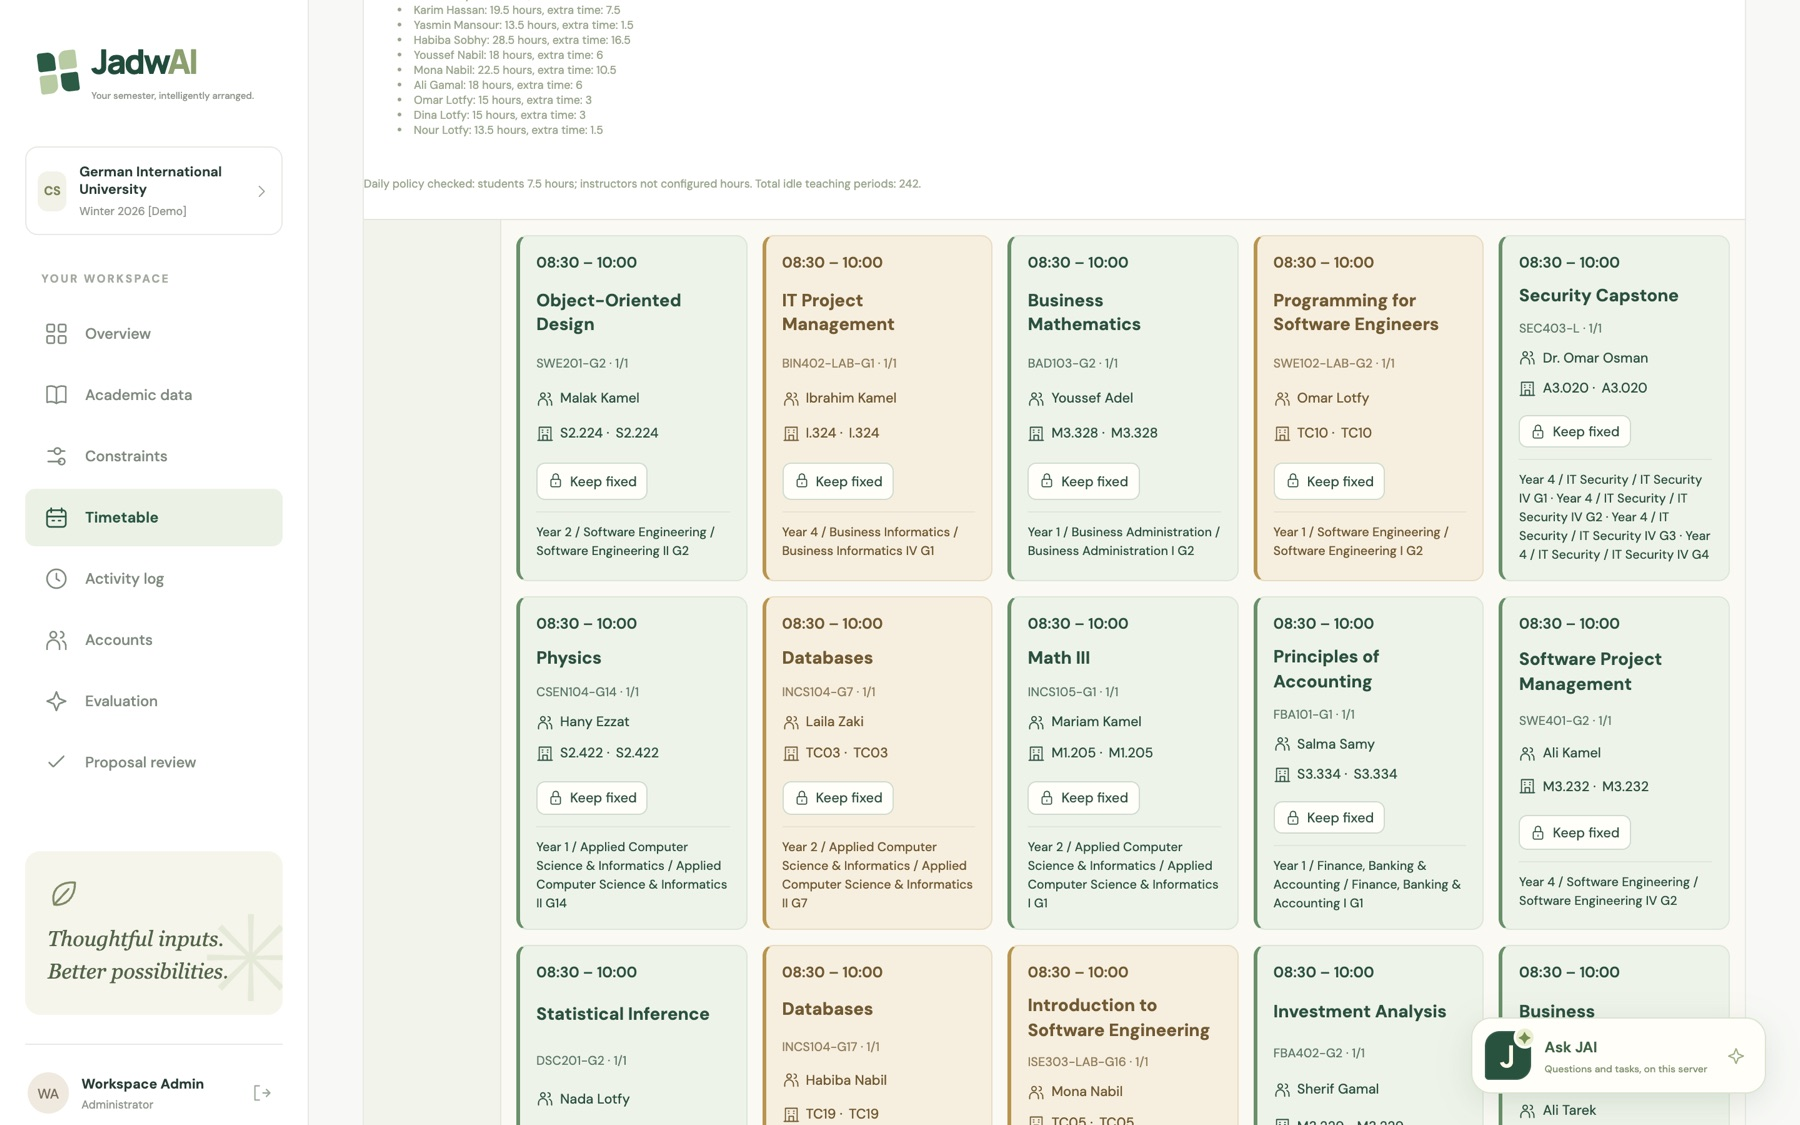
\includegraphics[width=\textwidth]{15-teaching-timetable-2.jpg}
\caption{Part of a published teaching timetable: each session shows time, course, activity, instructor and room, with an option to keep it fixed in later regenerations.}
\label{fig:shot-teaching-timetable-2}
\end{figure}

\begin{figure}[p]
\centering
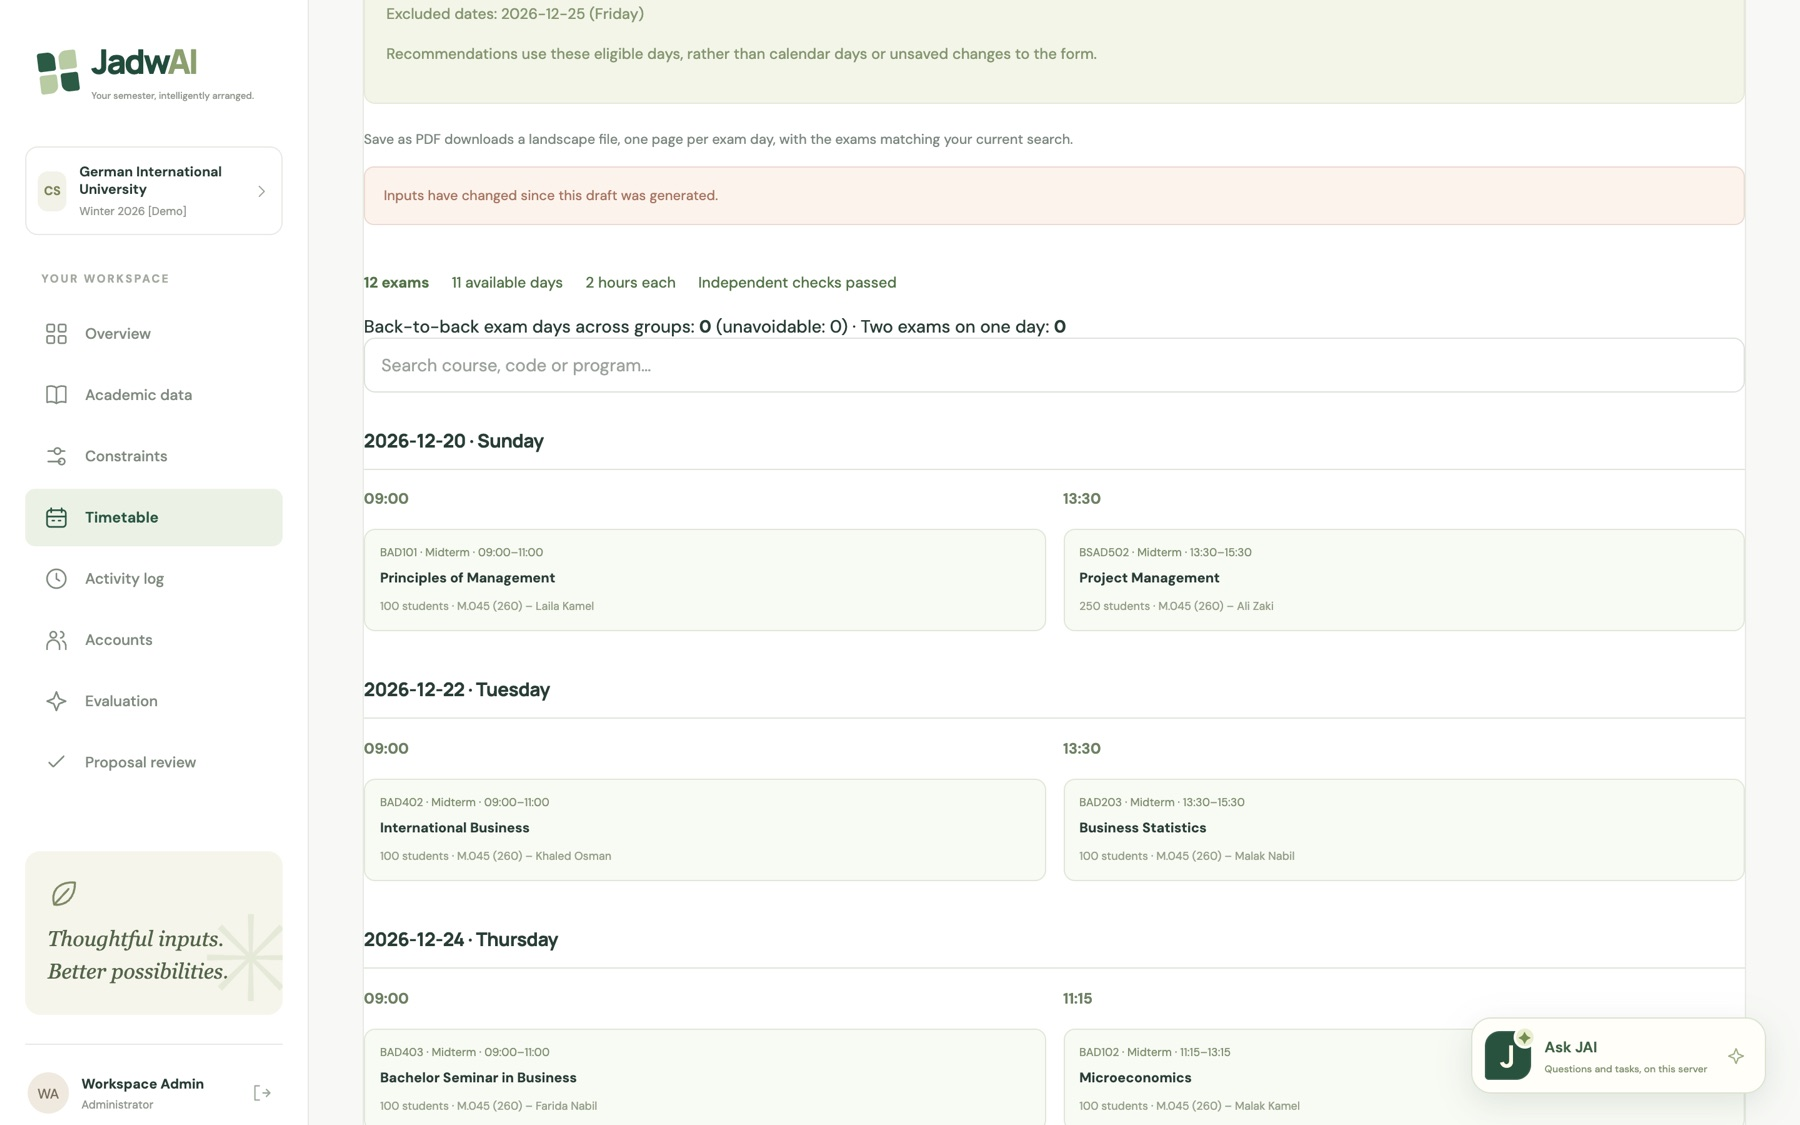
\includegraphics[width=\textwidth]{16-exam-timetable.jpg}
\caption{Examination timetable: midterms by day and time with hall, capacity and invigilator; the summary reports back-to-back examination days across groups.}
\label{fig:shot-exam-timetable}
\end{figure}

\begin{figure}[p]
\centering
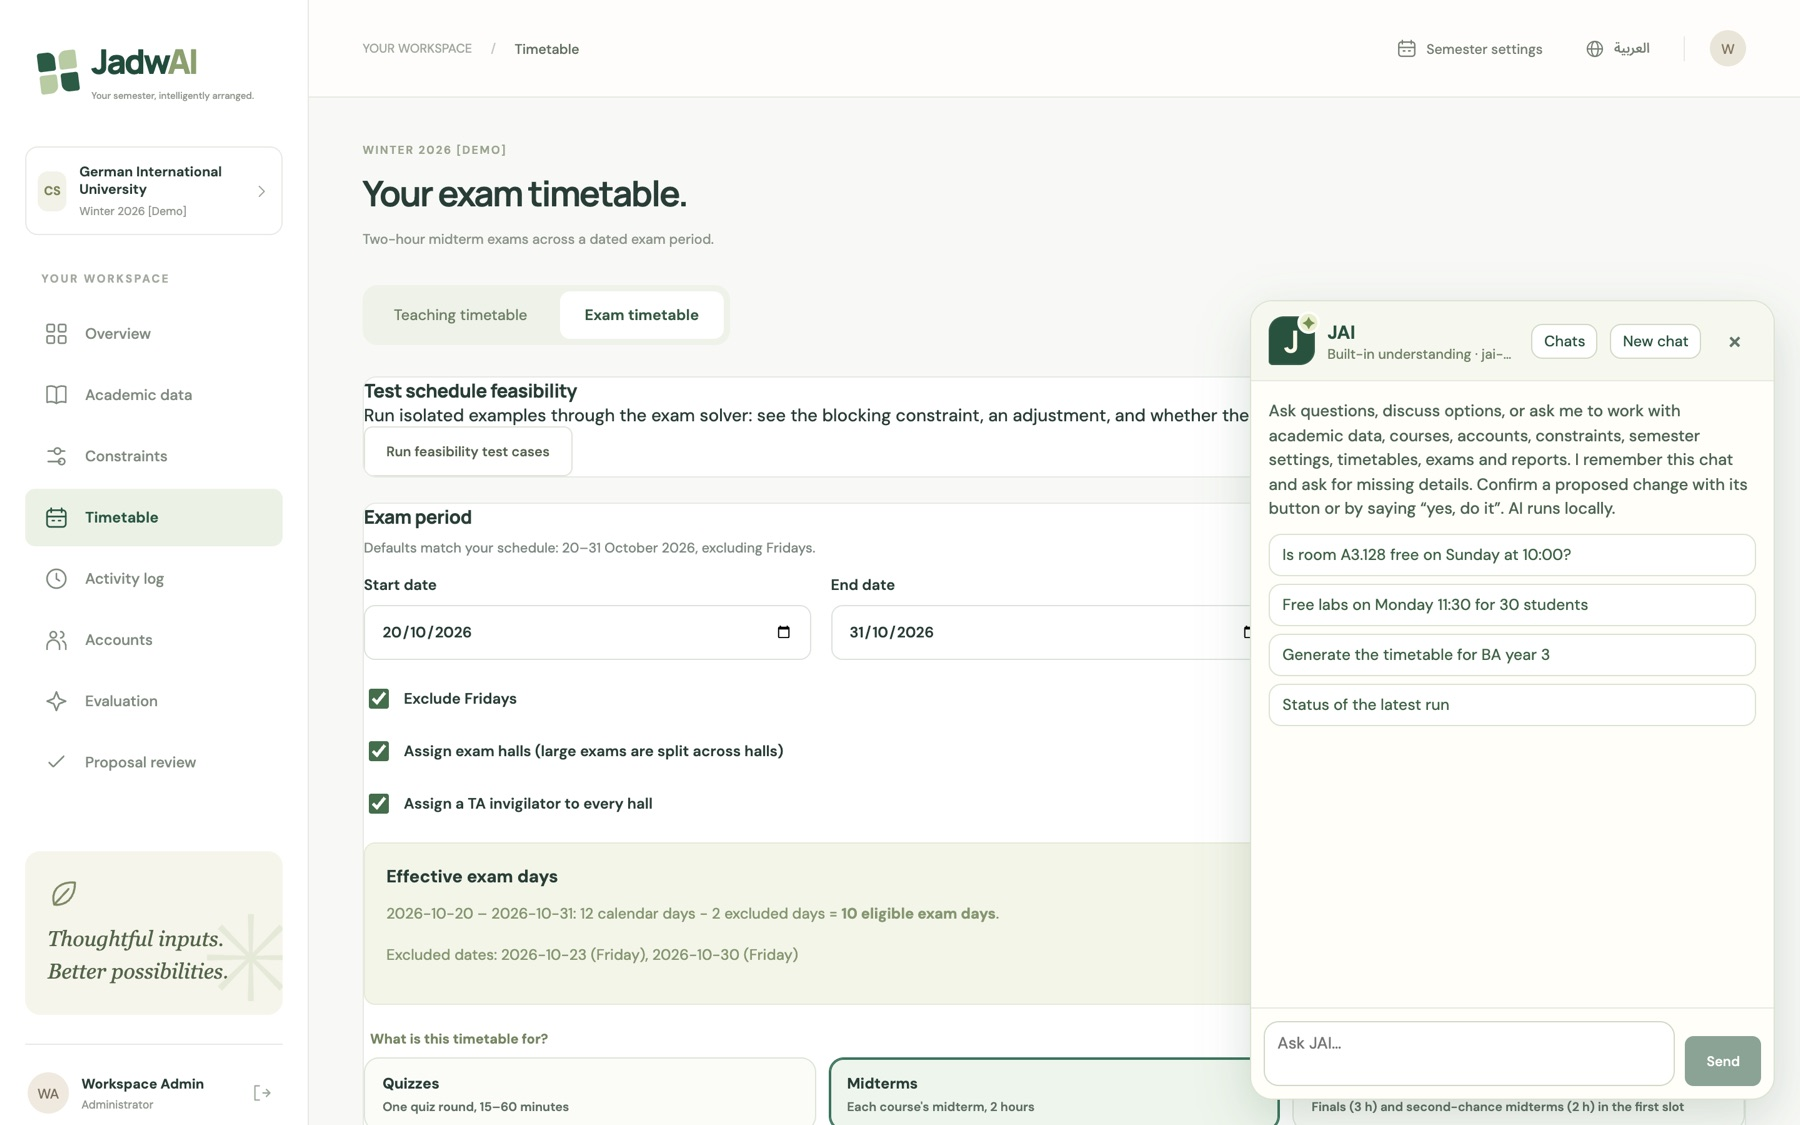
\includegraphics[width=\textwidth]{18-jai-chat.jpg}
\caption{The JAI chat panel beside the exam settings: example questions and tasks; a proposed change runs only after the administrator confirms it.}
\label{fig:shot-jai-chat}
\end{figure}

\begin{figure}[p]
\centering
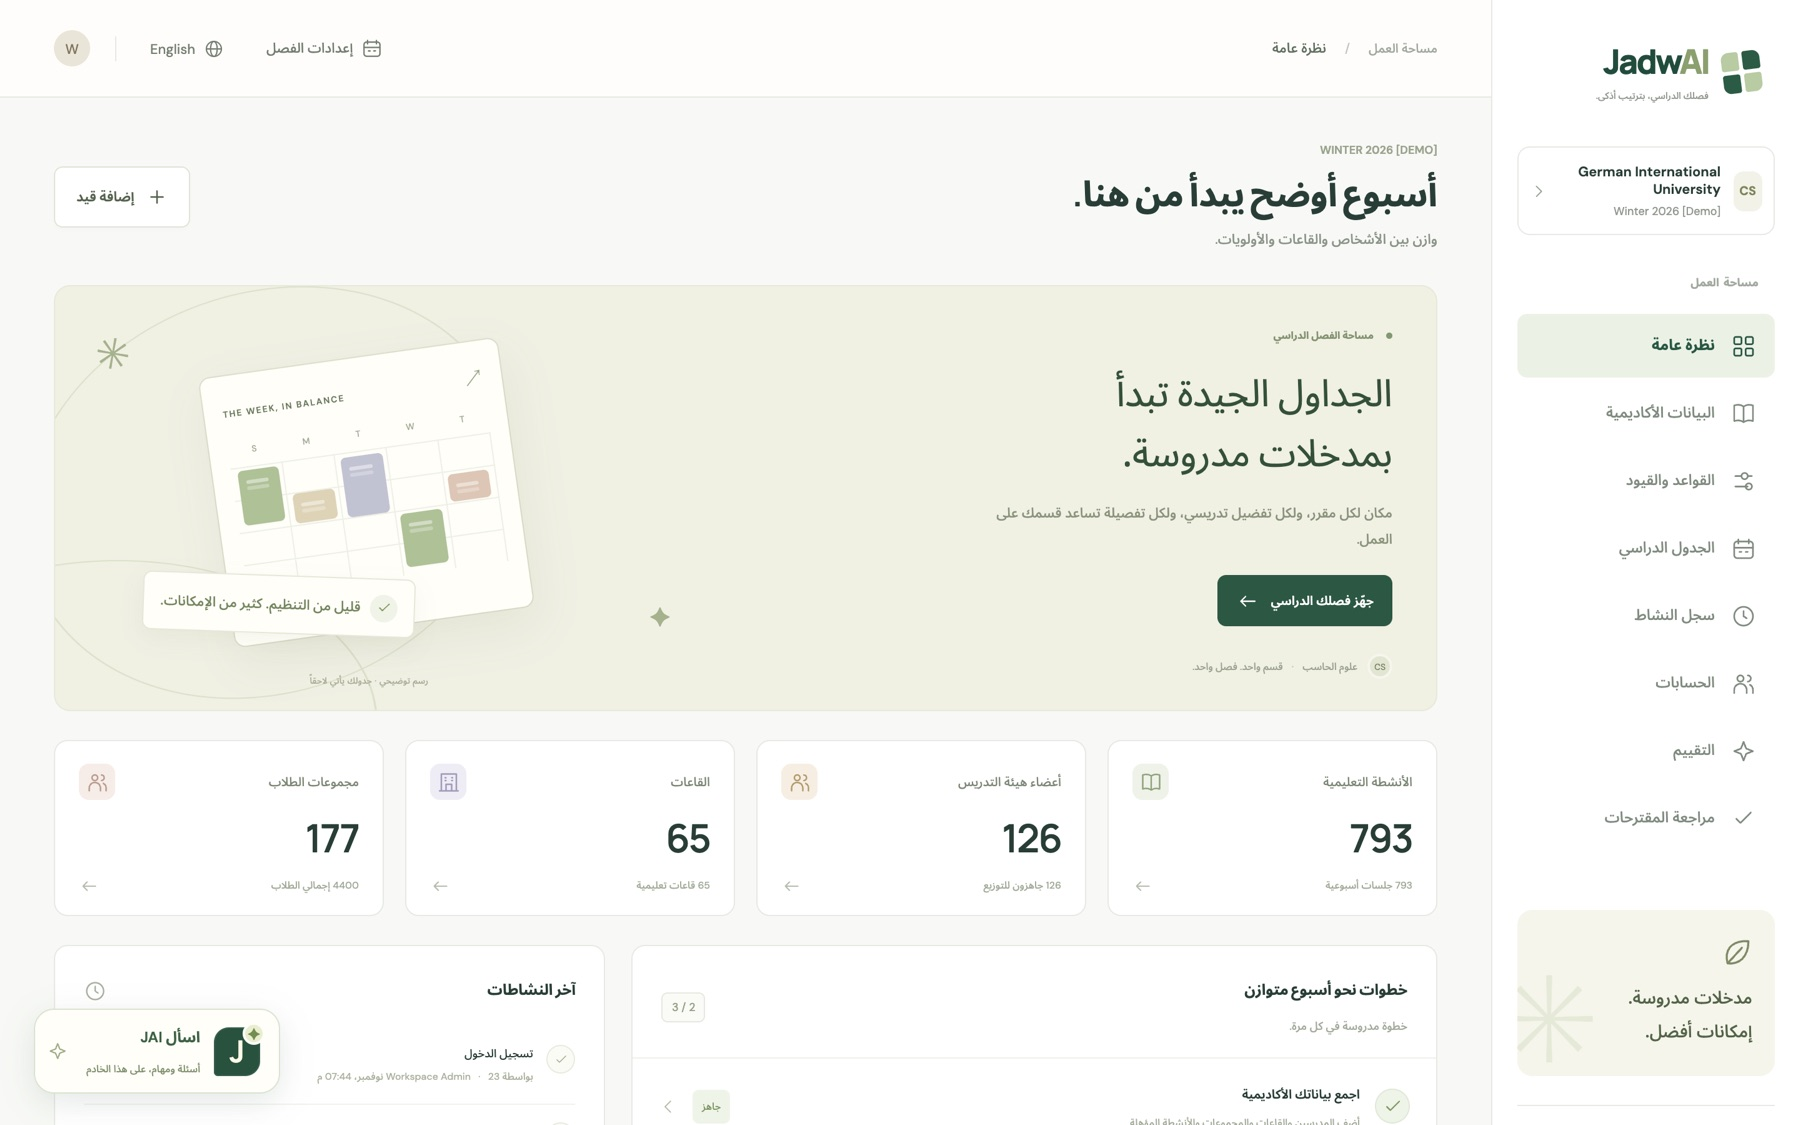
\includegraphics[width=\textwidth]{11-overview-arabic.jpg}
\caption{Arabic interface: the same overview page with right-to-left layout.}
\label{fig:shot-overview-arabic}
\end{figure}

\begin{figure}[p]
\centering
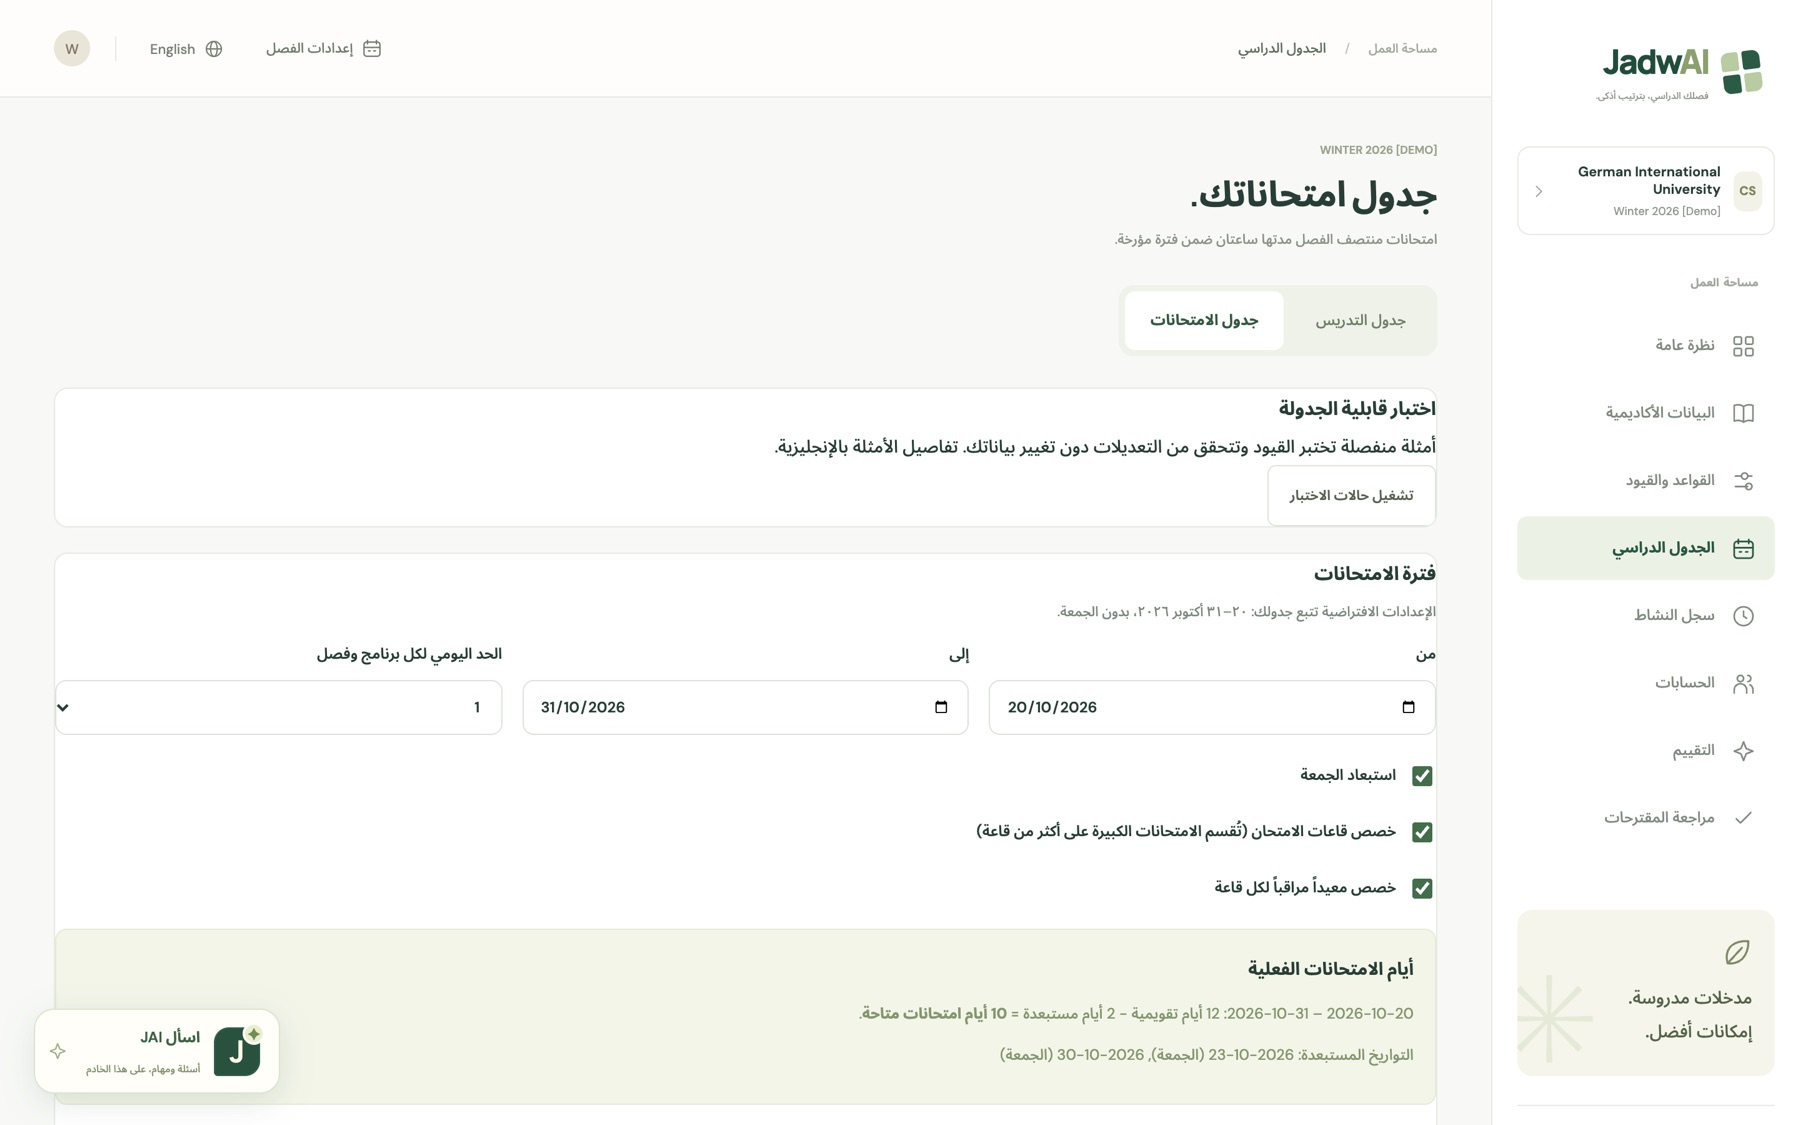
\includegraphics[width=\textwidth]{12-timetable-arabic.jpg}
\caption{Arabic interface: the examination settings page.}
\label{fig:shot-timetable-arabic}
\end{figure}

\clearpage

\chapter{Planning Records from the Proposal}\label{app:planning}

% NOTE (migration 23 Nov 2026): Text moved unchanged from main.tex. Much of it was drafted with AI assistance; rewrite it in your own words before submission (the supervisor runs AI checks).
% NOTE (migration 23 Nov 2026): These sections came from the proposed-methodology chapter. Keep only what still helps the reader, or remove this appendix.
\hypertarget{timeline}{%
\section{Timeline}\label{timeline}}

No deadline has been provided, so no dates are proposed (OQ-14). The
order of work is set out in SRS Section\textasciitilde16 and refined in a
current phased implementation roadmap that places
the annotation guide and evaluation data before AI extraction.

\hypertarget{proposed-deliverables-of-the-study}{%
\section{Proposed deliverables of the
study}\label{proposed-deliverables-of-the-study}}

Constraint vocabulary and schema; annotation guide; annotated dataset
(shareable portion, if permitted); frozen prompts and configurations;
raw outputs; analysis scripts; results with limitations; the prototype;
the thesis.

\hypertarget{consistency-with-the-srs-traceability}{%
\section{Consistency with the SRS
(traceability)}\label{consistency-with-the-srs-traceability}}

\begin{longtable}[]{@{}p{\dimexpr(\linewidth-4\tabcolsep)/2\relax}p{\dimexpr(\linewidth-4\tabcolsep)/2\relax}@{}}
\toprule\noalign{}
Methodology element & Specified feature or research procedure \\
\midrule\noalign{}
\endhead
\bottomrule\noalign{}
\endlastfoot
Extraction with schema-constrained output & FR-015, FR-022 \\
Entity resolution; invented entities & FR-016 \\
Parameters, named periods & FR-001, FR-017 \\
Negation, polarity, hard/soft & FR-018 \\
Clarification and unsupported handling & FR-019 \\
Review; raw versus post-review & FR-020 (stores raw and approved) \\
Approval gate & FR-021 \\
Experiment harness; metrics incl. paraphrase and run-to-run consistency;
versioned development records; frozen held-out configuration; held-out
isolation and access log & FR-049 \\
Annotator rating of clarification-question usefulness; inter-annotator
agreement; sample-size and statistics & research procedures
(dataset/analysis), no FR \\
Audit of model, prompt, cost, latency & FR-023 \\
Manual-entry baseline & FR-010 \\
Manual versus assisted timing and corrections & FR-050 \\
Scheduling measures & FR-024--FR-029, FR-031 \\
Seeded-violation and differential tests of the validator & FR-031 (SRS
EV-7; research procedure) \\
Coverage statements & FR-030, FR-032 \\
System-behaviour tests & SRS AC-01--AC-23 \\
Concurrent changes and publication consistency & FR-059; AC-16 \\
Interrupted operations and recovery & FR-060; AC-17 \\
Duplicate requests and bounded retries & FR-061; AC-18 \\
Incomplete results and cancellation completion & FR-062; AC-19 \\
Validator failures and publication blocking & FR-063; AC-20 \\
Session expiry and permission changes & FR-064; AC-21 \\
Reproducibility records & FR-023--FR-025, FR-046; NFR-016 \\
Differential testing against the solver model & research procedure
(Section\textasciitilde3.11); requires the validator and model to be
separately callable (NFR-002) \\
Rule-based baseline (optional) & research procedure; \textbf{no FR} ---
it is a test-time artefact, not a product feature \\
\end{longtable}

Instructor eligibility, locks and continuity are covered by AC-22; four-language input and the bilingual RTL interface by AC-23. These identifiers refer to the revised scope and do not imply that the older exported SRS has been synchronised. Fixed-assignment solver/validator cross-checks must fix instructor variables too. Infeasibility reporting provides available conflict details; automatic repair remains deferred.

Items marked "research procedure" are deliberately not product
requirements. Every other evaluated capability has an FR.

\hypertarget{decisions-needed-to-finalise-this-chapter}{%
\section{Decisions needed to finalise this
chapter}\label{decisions-needed-to-finalise-this-chapter}}

The remaining decisions concern complete constraint semantics; university template and length; dataset source, size and annotators; success targets; participant study and ethics; model selection and approved cost cap; data/provider policy; institutional workload values and additional daily-limit variants; partial diagnostic result sources; and the submission deadline. Exams, language scope, group-based conflict checking and elapsed-teaching-hour units have been resolved as stated in Chapter~1. The citation style has been resolved as IEEE (BibTeX style \texttt{ieeetr}, numbered in order of first citation). The initial corpus remains unreviewed, so its current size and labels do not resolve the final research sampling or annotation decisions.
